%!TEX TS-program = pdflatex
%!TEX root = ../main.tex
%!TEX encoding = UTF-8 Unicode


\section[Section]{Section}

\subsection[Subsection]{System design}

\begin{frame}{Use Case Diagram}
	The first step of our development to identify the use cases of our system.
	We have identified four main use cases:

	\begin{figure}[h!]
		\centering
		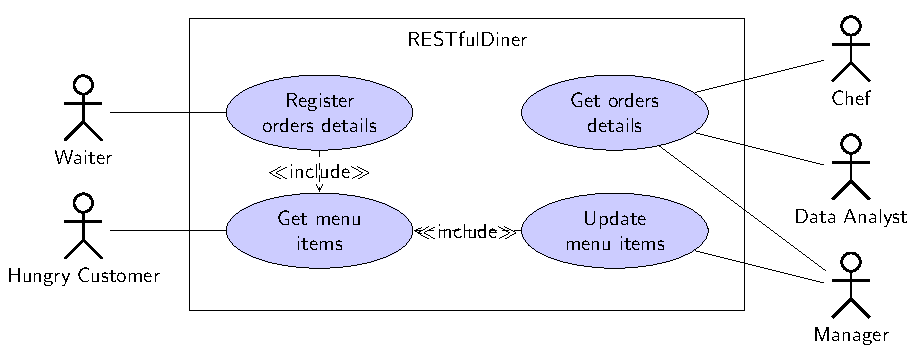
\includegraphics[width=0.9\textwidth,height=0.75\textheight,keepaspectratio]{images/usecases}
		\caption{Use cases diagram}
		\label{fig:usecases}
	\end{figure}

\end{frame}

\begin{frame}{E/R Diagram}
	\begin{figure}[h!]
		\centering
		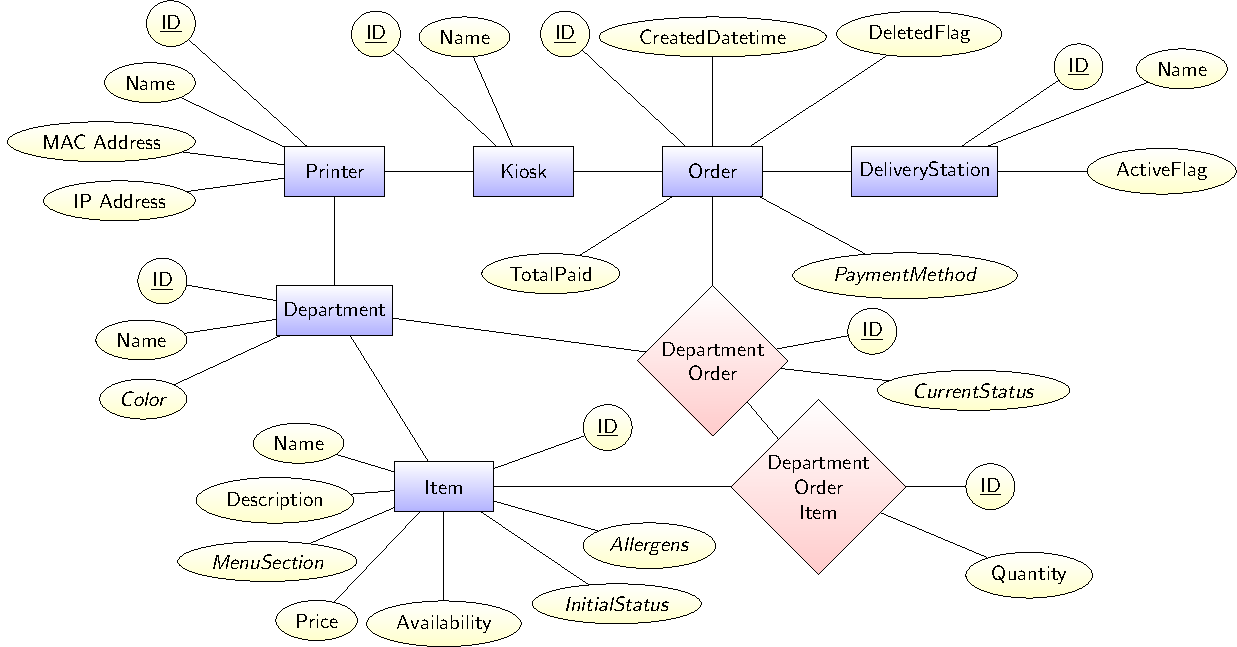
\includegraphics[width=\textwidth,height=0.75\textheight,keepaspectratio]{images/er}
		\caption{E/R diagram}
		\label{fig:er}
	\end{figure}

\end{frame}
